\documentclass[12pt,a4paper]{article}

% Language and encoding
\usepackage[T1]{fontenc}
\usepackage[utf8]{inputenc}
\usepackage[polish]{babel}

% Page layout
\usepackage[margin=2.5cm]{geometry}
\usepackage{fancyhdr}
\usepackage{graphicx}
\graphicspath{{SPRAWOZDANIE/}{./}}  % dziala z katalogu glownego repo i z katalogu SPRAWOZDANIE
\usepackage{float}
\usepackage{caption}

% Block diagrams
\usepackage{tikz}
\usetikzlibrary{positioning, arrows.meta, calc}

% Tables and content
\usepackage{array}
\usepackage{tabularx}
\usepackage{booktabs}
\usepackage{multirow}
\usepackage{xcolor}
\usepackage{colortbl}

% Math and equations
\usepackage{amsmath}
\usepackage{amssymb}
\usepackage{amsfonts}

% Lists and spacing
\usepackage{enumitem}
\usepackage{setspace}
\onehalfspacing

% Hyperlinks
\usepackage{hyperref}
\hypersetup{colorlinks=true, linkcolor=black, urlcolor=blue}

% Syntax highlighting %
\usepackage{listings}
\lstset{
    language=Verilog,
    numbers=left,
    numberstyle=\tiny\color{gray},
    stepnumber=1,
    numbersep=8pt,
    backgroundcolor=\color{gray!5}, % Delikatne tło
    frame=single,                   % Ramka wokół kodu
    frameround=ffff,
    rulecolor=\color{gray!30},
    keywordstyle=\color{blue}\bfseries,
    commentstyle=\color{green!60!black},
    stringstyle=\color{purple},
    basicstyle=\ttfamily\small,
    breaklines=true,
    showstringspaces=false
}

% Centered fixed-width column macro
\newcolumntype{C}[1]{>{\centering\arraybackslash}m{#1}}

% Logic operator macros (AND / OR)
\providecommand{\und}{\land}
\providecommand{\oder}{\lor}

% Highlight macro for masked faults (signature identical to the golden one)
\newcommand{\dc}[1]{\cellcolor{red!18}\textbf{#1}}

% ===== DOCUMENT SETUP =====
\title{}
\author{}
\date{}

\pagestyle{fancy}
\fancyhf{}
\rfoot{\thepage}
\renewcommand{\headrulewidth}{0pt}

\begin{document}

% ===== TITLE PAGE =====
\begin{titlepage}
    \centering

    % Logo
    
\includegraphics[width=5cm]{logo.png}
    \vspace{1cm}

    % Header
    {\Large \textbf{WYDZIAŁ AUTOMATYKI, ELEKTRONIKI I INFORMATYKI}}

    \vspace{2cm}

    % Laboratory title
    {\large \textbf{Laboratorium}}

    {\large \textbf{System on Chip}}

    \vspace{2cm}

    {\large \textbf{Sprawozdanie}}

    \vspace{1cm}

    % Exercise number and title

    {\LARGE \textbf{Projekt}}

    \vspace{1cm}

    {\LARGE \textbf{Zegar Dot Matrix}}

    \vspace{2cm}

    % Author and details
    \raggedright
    \large
    Autor: \textbf{Bartosz Faruga}

    \vspace{0.5cm}

    Rok akademicki 2025/2026, semestr 1

    \vspace{1cm}

    \centering
    Gliwice, \today

\end{titlepage}

\newpage

\setcounter{tocdepth}{2}
% \tableofcontents
% \newpage

% =====================================================================
\section{Idea projektu}

Celem projektu było zbudowanie cyfrowego zegara z~funkcją budzika, którego
elementem wyświetlającym jest matryca diod LED typu \emph{dot-matrix}
złożona z~czterech kaskadowo połączonych modułów 8$\times$8 sterowanych
układami MAX7219. Całość zrealizowano jako system SoC (\emph{System on
Chip}) na układzie Xilinx Zynq-7020 (płyta ZedBoard), wykorzystując oba
podsystemy tego układu:

\begin{itemize}[noitemsep]
    \item \textbf{PS} (\emph{Processing System}) -- rdzeń ARM Cortex-A9,
          na którym działa oprogramowanie sterujące zegara (logika
          aplikacji, zegar czasu rzeczywistego, obsługa klawiatury);
    \item \textbf{PL} (\emph{Programmable Logic}) -- część FPGA, w~której
          zaimplementowano sprzętowy dekoder znaków ASCII oraz silnik
          szeregowej transmisji danych do układów MAX7219.
\end{itemize}

Podział zadań pomiędzy oba podsystemy wynika wprost z~wymagań projektu i~jest
zestawiony w~tabeli~\ref{tab:wymagania}. Część czasowo-krytyczna i~powtarzalna
(generowanie ramek szeregowych, dekodowanie ASCII$\rightarrow$piksele) trafiła
do logiki programowalnej, natomiast logika sterująca o~charakterze sekwencyjnym
(tryby pracy, nastawianie czasu, antydrganiowa obsługa przycisków, RTC) --
do oprogramowania rdzenia ARM. Silnik szeregowy MAX7219 został wstępnie
uruchomiony na osobnej, tańszej płycie prototypowej Tang Nano~9K (FPGA Gowin
GW1NR-9), a~dopiero po weryfikacji przeniesiony do układu Zynq.

\begin{table}[H]
\centering
\caption{Wymagania projektowe i~miejsce ich realizacji.}
\label{tab:wymagania}
\small
\begin{tabularx}{\textwidth}{@{}p{5.2cm} c X@{}}
\toprule
\textbf{Wymaganie} & \textbf{Domena} & \textbf{Realizacja} \\
\midrule
Dekodowanie ASCII na dane MAX7219 & PL & \texttt{font\_rom} + \texttt{translator} \\
Szeregowa transmisja na matrycę    & PL & \texttt{dot\_matrix\_fifo} (silnik SPI) \\
Transpozycja kolumny$\rightarrow$wiersz & PL & wysyłanie po wierszach (rejestry cyfr) \\
Miganie wybranego znaku            & PL/PS & rejestr \texttt{blink} + wygaszanie w~firmware \\
Przerwania RTC                     & PL/PS & timer z~linią IRQ + ISR \\
Antydrgania i~autopowtarzanie      & PS & \texttt{keyboard.h} \\
Zegar czasu rzeczywistego          & PS & \texttt{rtc.h} (przerwanie 1~Hz) \\
Tryby pracy: czas / alarm          & PS & \texttt{clock\_app.h} \\
\bottomrule
\end{tabularx}
\end{table}

\clearpage
% =====================================================================
\section{Struktura} % o części fpga

System składa się z~rdzenia ARM (PS) komunikującego się z~logiką programowalną
(PL) poprzez magistralę AXI4-Lite. Całość spięto w~jednym module
najwyższego poziomu \texttt{ZED\_IRQ}, w~którym rdzeń \texttt{PS7} jest
\emph{instancjonowany bezpośrednio w~Verilogu} (bez użycia integratora bloków),
a~jego port nadrzędny \texttt{M\_AXI\_GP0} dołączono wprost do
slave'a AXI4-Lite \texttt{AXI\_IO\_INT} udostępnionego przez prowadzącego. Procesor zapisuje w~ten sposób do
rejestrów peryferium zakodowaną w~ASCII treść do wyświetlenia oraz rozkazy
sterujące; logika dekoduje te dane i~steruje fizycznie matrycą LED, a~zwrotnie
zgłasza do procesora przerwanie timera. Ogólną architekturę przedstawia
rys.~\ref{fig:arch}.

\begin{figure}[H]
\centering
\begin{tikzpicture}[
    node distance=1.5cm and 1.4cm,
    every node/.style={font=\small},
    box/.style={draw, rounded corners, align=center, minimum height=1.6cm,
                text width=3.2cm, fill=gray!8},
    flow/.style={-{Latex[length=2.5mm]}, thick}]
  % --- gorny wiersz: PS7 -> AXI_IO_INT -> state_machine ---
  \node[box] (ps)   {Zynq \texttt{PS7}\\Cortex-A9\\\footnotesize M\_AXI\_GP0 / IRQF2P};
  \node[box, right=of ps]  (axi)  {\texttt{AXI\_IO\_INT}\\slave AXI4-Lite\\\footnotesize rejestry + timer};
  \node[box, right=of axi] (sm)   {\texttt{FSM}};
  \node[box, above=of sm] (tr)   {\texttt{Translator}};
  \node[box, above=of tr] (ram)   {\texttt{BRAM}};
  % --- dolny wiersz (powrotny): SPI -> matryca ---
  \node[box, below=of sm]   (spi) {\texttt{dot\_matrix\_fifo}\\silnik SPI};
  \node[box, left=of spi]   (disp){4$\times$ MAX7219\\matryca 8$\times$8};

  \draw[flow] (ps)   -- node[above,font=\footnotesize]{GP0} (axi);
  \draw[flow] (axi)  -- node[above,align=center,font=\footnotesize]{ascii\\ctrl} (sm);
  \draw[flow] (sm)   -- node[right,align=center,font=\footnotesize]{packet} (spi);
  \draw[flow] (tr)   -- node[right,align=center,font=\footnotesize]{row\\packet} (sm);
  \draw[flow] (ram)   -- node[right,align=center,font=\footnotesize]{ascii\\row} (tr);
  \draw[flow] (spi)  -- node[midway,above,align=center,font=\footnotesize]{SCLK\\CS\\DIN} (disp);
  % --- zwrotna linia przerwania timera, poprowadzona ponad ukladem ---
  \draw[flow] (axi.north) to[out=90,in=90,looseness=0.9]
        node[above,font=\footnotesize]{IRQ 1~Hz (timer)} (ps.north);
\end{tikzpicture}
\caption{Architektura SoC}
\label{fig:arch}
\end{figure}

\subsection{PS} % o części cpp

Oprogramowanie rdzenia ARM napisano w~języku C w~konwencji \emph{header-only}
(każdy moduł to samodzielny nagłówek dołączany w~jednej jednostce kompilacji).
Strukturę kodu i~odpowiedzialność modułów zestawiono w~tabeli~\ref{tab:ps}.

\begin{table}[H]
\centering
\caption{Moduły oprogramowania PS.}
\label{tab:ps}
\small
\begin{tabularx}{\textwidth}{@{}l X@{}}
\toprule
\textbf{Plik} & \textbf{Zadanie} \\
\midrule
\texttt{zybo\_int.c} & punkt wejścia: inicjalizacja GIC i~podsystemów, pętla główna \\
\texttt{config.h}    & mapa rejestrów sprzętowych i~stałe konfiguracyjne \\
\texttt{rtc.h}       & zegar czasu rzeczywistego oparty o~przerwanie 1~Hz \\
\texttt{keyboard.h}  & antydrgania i~autopowtarzanie 5~przycisków \\
\texttt{display.h}   & sterownik matrycy MAX7219 ponad rejestrami AXI \\
\texttt{clock\_app.h}& automat stanów interfejsu użytkownika (tryby, alarm) \\
\bottomrule
\end{tabularx}
\end{table}

Program nie używa systemu operacyjnego -- działa w~modelu \emph{bare-metal}.
Po inicjalizacji kontrolera przerwań (GIC), timera RTC, klawiatury
i~wyświetlacza wykonywana jest nieskończona pętla odpytująca (\emph{poll
loop}) o~stałym okresie \texttt{POLL\_MS}~$=10$~ms (listing~\ref{lst:main}).
W~każdej iteracji próbkowane są przyciski, obsługiwane jest zdarzenie sekundowe
generowane przez przerwanie RTC oraz odświeżany jest stan wyświetlacza.

\begin{lstlisting}[language=C, caption={Pętla główna (\texttt{zybo\_int.c}).}, label={lst:main}]
for (;;) {
    app_handle_buttons(kb_scan());      // antydrgania + autorepeat
    if (rtc_take_sec_event())           // flaga ustawiana w ISR timera
        app_second_tick();              // dopasowanie alarmu co 1 s
    app_refresh();                      // miganie + render na matrycy
    usleep(POLL_MS * 1000);
}
\end{lstlisting}

Sam zegar realizowany jest przez przerwanie sprzętowego timera o~częstotliwości
1~Hz (wektor GIC nr~61). Procedura obsługi przerwania (listing~\ref{lst:rtc})
kasuje flagę przerwania, inkrementuje liczniki sekund/minut/godzin i~ustawia
flagę \texttt{rtc\_sec\_event}, którą pętla główna konsumuje raz na sekundę.
Odczyt i~zapis czasu wykonywany jest przy chwilowo zamaskowanym przerwaniu,
co eliminuje ryzyko odczytu niespójnego (\emph{tearing}).

\begin{lstlisting}[language=C, caption={Procedura obsługi przerwania RTC (\texttt{rtc.h}).}, label={lst:rtc}]
static void rtc_isr(void *cb) {
    rtc_tm->tmCTRL = (1u << TM_INT) | (1u << TM_RUN);  // skasuj IRQ, timer dalej liczy
    if (++rtc_ss >= 60) { rtc_ss = 0;
        if (++rtc_mm >= 60) { rtc_mm = 0;
            if (++rtc_hh >= 24) rtc_hh = 0; } }
    rtc_sec_event = 1;
}
\end{lstlisting}

Obsługa klawiatury (\texttt{keyboard.h}) realizuje dwa wymagane mechanizmy.
\textbf{Antydrgania}: stan przycisku zmienia się dopiero po
\texttt{DEBOUNCE\_TICKS}~$=3$ kolejnych identycznych próbkach (30~ms).
\textbf{Autopowtarzanie}: przytrzymanie przycisku przez
\texttt{REPEAT\_DELAY}~$=500$~ms uruchamia powtórzenia co
\texttt{REPEAT\_PERIOD}~$=120$~ms. Każdy przycisk ma własny, niezależny stan
(struktura \texttt{Btn}), a~funkcja \texttt{kb\_scan()} zwraca maskę zdarzeń
do dalszego przetworzenia przez automat aplikacji.

\subsection{PL}

Część logiki programowalnej opisano w~języku Verilog. Hierarchię modułów oraz
ich rolę zestawiono w~tabeli~\ref{tab:pl}. Modułem nadrzędnym jest
\texttt{state\_machine} -- automat sterujący, który na podstawie rejestru
rozkazów wykonuje sekwencje wysyłane do matrycy. Cała logika sterowania matrycą
taktowana jest wolniejszym sygnałem z~\texttt{clock\_div} (100~MHz dzielone
przez~10), dzięki czemu wynikowy zegar szeregowy SCLK nie przekracza
dopuszczalnych dla MAX7219 10~MHz.

\begin{table}[H]
\centering
\caption{Moduły logiki programowalnej (PL).}
\label{tab:pl}
\small
\begin{tabularx}{\textwidth}{@{}l X@{}}
\toprule
\textbf{Moduł} & \textbf{Zadanie} \\
\midrule
\texttt{state\_machine} & automat główny: inicjalizacja, jasność, render ASCII \\
\texttt{translator} & dla danego wiersza pobiera piksele 4~znaków i~składa ramkę \\
\texttt{font\_rom}  & ROM czcionki: kod ASCII (7~b) $\rightarrow$ bitmapa 8$\times$8 \\
\texttt{dot\_matrix\_fifo} & silnik szeregowy (SPI) sterujący MAX7219 \\
\texttt{clock\_div} & podział 100~MHz\,/\,10 -- takt \texttt{state\_machine} (SCLK $\le$10~MHz) \\
\bottomrule
\end{tabularx}
\end{table}

\textbf{Silnik szeregowy.} Moduł \texttt{dot\_matrix\_fifo} implementuje
protokół MAX7219: 16-bitowe słowa wysyłane bitem najstarszym (MSB) naprzód,
gdzie DIN próbkowane jest na zboczu narastającym SCLK. Dla $N=4$ kaskadowo
połączonych układów wysyłane jest $N\times16=64$~bity przy aktywnym (niskim)
sygnale CS/LOAD, po czym zbocze narastające CS zatrzaskuje wszystkie słowa
jednocześnie. Automat (stany \texttt{IDLE}/\texttt{SHIFT}/\texttt{LATCH})
sygnalizuje zajętość linią \texttt{busy}; dostępne jest też wejście
\texttt{abort} pozwalające natychmiast przerwać bieżącą ramkę. Format słowa
sterującego MAX7219 to: bity [11:8] -- adres rejestru, [7:0] -- dane.
Najważniejsze rozkazy konfiguracyjne zestawia tabela~\ref{tab:max}.

\begin{table}[H]
\centering
\caption{Słowa konfiguracyjne MAX7219 użyte w~sekwencji inicjalizacji.}
\label{tab:max}
\small
\begin{tabularx}{\textwidth}{@{}l l X@{}}
\toprule
\textbf{Słowo} & \textbf{Rejestr} & \textbf{Znaczenie} \\
\midrule
\texttt{0x0C01} & shutdown    & wyjście ze stanu uśpienia (praca normalna) \\
\texttt{0x0B07} & scan-limit  & skanowanie wszystkich 8~wierszy \\
\texttt{0x0900} & decode mode & brak dekodowania (surowe segmenty) \\
\texttt{0x0A0n} & intensity   & jasność (sterowana z~PS, poziomy 0--3) \\
\bottomrule
\end{tabularx}
\end{table}

\textbf{Dekodowanie i~transpozycja.} Wymaganie „transpozycji z~zapisu
kolumnowego na wyświetlanie wierszowe” zrealizowano przez wysyłanie obrazu
\emph{wiersz po wierszu}. Dla wiersza $r$ moduł \texttt{translator} pobiera
z~\texttt{font\_rom} 8-bitowy wzór tego wiersza dla każdego z~4~znaków i~składa
ramkę 4$\times$16~b, w~której każde słowo adresuje rejestr cyfry MAX7219
($r{+}1$, bo rejestry numerowane są 1--8) -- listing~\ref{lst:trans}. Automat
\texttt{state\_machine} powtarza to dla wszystkich 8~wierszy, dając kompletne
odświeżenie wyświetlacza w~8~ramkach szeregowych.

\begin{lstlisting}[language=Verilog, caption={Złożenie słowa ramki w~module \texttt{translator}.}, label={lst:trans}]
// rejestry cyfr MAX7219 numerowane 1..8, wiec adres = row_idx + 1
row_packet[(N-1-idx)*16 +: 16] <= {4'b0000, ({1'b0,row_idx} + 4'd1), row_data};
\end{lstlisting}

\subsection{AXI Lite} % połączenie

Komunikację PS$\leftrightarrow$PL zrealizowano przez magistralę AXI4-Lite, lecz
-- inaczej niż w~typowym przepływie z~integratorem bloków -- bez gotowych
rdzeni IP. Rdzeń \texttt{PS7} jest instancjonowany ręcznie w~module
\texttt{ZED\_IRQ}, a~jego port nadrzędny \texttt{M\_AXI\_GP0} dołączono wprost
do slave'a \texttt{AXI\_IO\_INT}. Moduł ten zawiera kompletne
automaty obsługi kanałów AXI4-Lite (zapis:
\texttt{W\_IDLE}$\rightarrow$\texttt{W\_WR}$\rightarrow$\texttt{W\_RESP};
odczyt: \texttt{R\_IDLE}$\rightarrow$\texttt{R\_DATA}$\rightarrow$\texttt{R\_DATA\_ACK}),
dekoduje adres transakcji na zestaw rejestrów (tab.~\ref{tab:regs}) i~udostępnia
logice sterującej sygnały \texttt{ASCII\_DATA} oraz \texttt{CTRL\_REG}. Zapis
rejestru obrazu honoruje maskę bajtów \texttt{WSTRB}, więc procesor może
modyfikować pojedyncze znaki. Wyjścia sterownika (\texttt{MAX\_CLK},
\texttt{MAX\_LOAD}, \texttt{MAX\_DIN}) wyprowadzono na złącze Pmod ZedBoard
(piny AA9 / AA11 / Y11).

\begin{table}[H]
\centering
\caption{Mapa rejestrów slave'a \texttt{AXI\_IO\_INT} (przestrzeń AXI~GP0).}
\label{tab:regs}
\small
\begin{tabularx}{\textwidth}{@{}l l c X@{}}
\toprule
\textbf{Rejestr} & \textbf{Adres} & \textbf{Dostęp} & \textbf{Opis} \\
\midrule
\texttt{ASCII\_DATA} & \texttt{0x40000000} & RW & 4~znaki $\times$ 7~b -- pamięć obrazu (z~\texttt{WSTRB}) \\
\texttt{CTRL\_REG}  & \texttt{0x40000004} & RW & rozkaz: [7:6]~op, [5]~kick, [1:0]~arg \\
\texttt{LED} (clr/tgl) & \texttt{0x08\,/\,0x0C} & W & dioda alarmu: zapis~1 zeruje\,/\,neguje bit \\
\texttt{SW}         & \texttt{0x40000020} & R  & przełączniki suwakowe \\
\texttt{PB}         & \texttt{0x40000024} & R  & 5~przycisków (L/R/D/U/C) \\
\texttt{TMR\_Q}     & \texttt{0x40000040} & RW & wartość przeładowania (start gdy $\ge$256) \\
\texttt{TMR\_CTRL}  & \texttt{0x40000044} & RW & START/STOP/RUN, flagi ZD\,(INT)/OV \\
\texttt{TMR\_CNT}   & \texttt{0x40000048} & R  & bieżący stan licznika \\
\bottomrule
\end{tabularx}
\end{table}

\textbf{Mechanizm „kick”.} Ponieważ rozkazy są przekazywane przez rejestr
(a~nie strumień danych), konieczne było rozróżnienie dwóch identycznych zapisów
następujących po sobie. Rozwiązano to bitem \texttt{kick} (bit~5
\texttt{ctrl\_reg}): firmware neguje go przy każdym zapisie
(listing~\ref{lst:kick}), a~logika wykrywa zbocze tego bitu, generując
jednotaktowy impuls \texttt{cmd\_valid}. Pozwala to ponawiać ten sam rozkaz
dowolną liczbę razy. Dodatkowo wejściowy \texttt{ctrl\_reg} jest synchronizowany
trzema przerzutnikami (CDC) przed użyciem, a~przyjście nowego rozkazu w~trakcie
trwającej transmisji powoduje jej przerwanie (\texttt{abort}) i~obsłużenie
nowego polecenia.

\begin{lstlisting}[language=C, caption={Wysyłanie rozkazu z~bitem „kick” (\texttt{display.h}).}, label={lst:kick}]
static inline void display_cmd(uint32_t op, uint32_t arg) {
    display_kick ^= 1u;                                   // negacja przy kazdym zapisie
    Xil_Out32(CTRL_REG, op | (display_kick << 5) | (arg & 3u));
}
\end{lstlisting}

\textbf{RTC i~przerwania.} Zegar czasu rzeczywistego opiera się o~timer
wbudowany w~\texttt{AXI\_IO\_INT}: licznik \texttt{TMR\_CNT} zlicza w~górę od~0
do wartości \texttt{TMR\_Q}, po czym zeruje się i~ustawia flagę przejścia przez
zero \texttt{ZD} (bit~31), będącą źródłem linii \texttt{IRQ}. Linia ta trafia
do wejścia \texttt{IRQF2P[0]} rdzenia \texttt{PS7}, co odpowiada przerwaniu
o~wektorze~61 w~kontrolerze GIC. Przy taktowaniu 100~MHz wartość
\texttt{TMR\_Q}~$=99\,999\,999$ daje przerwanie dokładnie raz na sekundę,
a~procedura obsługi kasuje flagę zapisem~1 na bit~31 rejestru sterującego.
Sam timer (z~flagami \texttt{ZD}/\texttt{OV} oraz warunkiem startu
\texttt{TMR\_Q}$\ge$256) pochodzi z~przykładu laboratoryjnego, rozszerzonego
na potrzeby projektu o~rejestry \texttt{ASCII\_DATA} i~\texttt{CTRL\_REG}.

\subsection{Pamięć ROM} % połączenie

\textbf{Blok pamięci czcionki (BRAM).} Moduł \texttt{font\_rom} odwzorowuje
7-bitowy kod ASCII (znaki \texttt{0x20}--\texttt{0x7E}) na bitmapę 8$\times$8
pikseli (64~bity). Adres znaku jest rejestrowany (\texttt{addr <= ascii\_code}),
a~odczyt wiersza odbywa się synchronicznie -- jest to klasyczny wzorzec
\emph{pamięci synchronicznej}, dzięki któremu narzędzie syntezy odwzorowuje
czcionkę na sprzętowy blok pamięci RAM (BRAM), a~nie na zasoby logiczne (LUT).
Wynikające stąd jednotaktowe opóźnienie odczytu jest ukryte przez stan
\texttt{WAIT\_ROM} modułu \texttt{translator}. Dzięki pełnemu zestawowi cyfr,
liter i~znaków ten sam wyświetlacz prezentuje zarówno czas (np. \texttt{12:30}),
jak i~komunikaty tekstowe.

\textbf{Pamięć obrazu.} Wymaganą „pamięć obrazu z~kodowaniem ASCII” oraz
„bezpośredni dostęp RW do pamięci wyświetlacza” realizuje rejestr
\texttt{ASCII\_DATA} w~\texttt{AXI\_IO\_INT}: firmware pakuje 4~znaki (po 7~bitów)
w~jedno 28-bitowe słowo makrem \texttt{PACK4} i~zapisuje je jednym dostępem AXI. Aby ograniczyć
ruch na magistrali, \texttt{display\_send()} buforuje ostatnio wysłaną
zawartość i~ponawia transmisję tylko przy faktycznej zmianie obrazu.

Efekt implementacji widać na widoku struktury krzemowej układu
(rys.~\ref{fig:fabric}): narzędzie rozmieściło logikę projektu w~komórkach
konfigurowalnych (CLB) -- zajęte przerzutniki i~tablice LUT zaznaczono kolorem
turkusowym -- obok regularnych, pionowych kolumn dedykowanych zasobów
(bloki pamięci BRAM oraz DSP). Pamięć czcionki \texttt{font\_rom} trafia
właśnie do takiego bloku BRAM, zamiast zajmować zasoby logiczne CLB.

\begin{figure}[H]
\centering
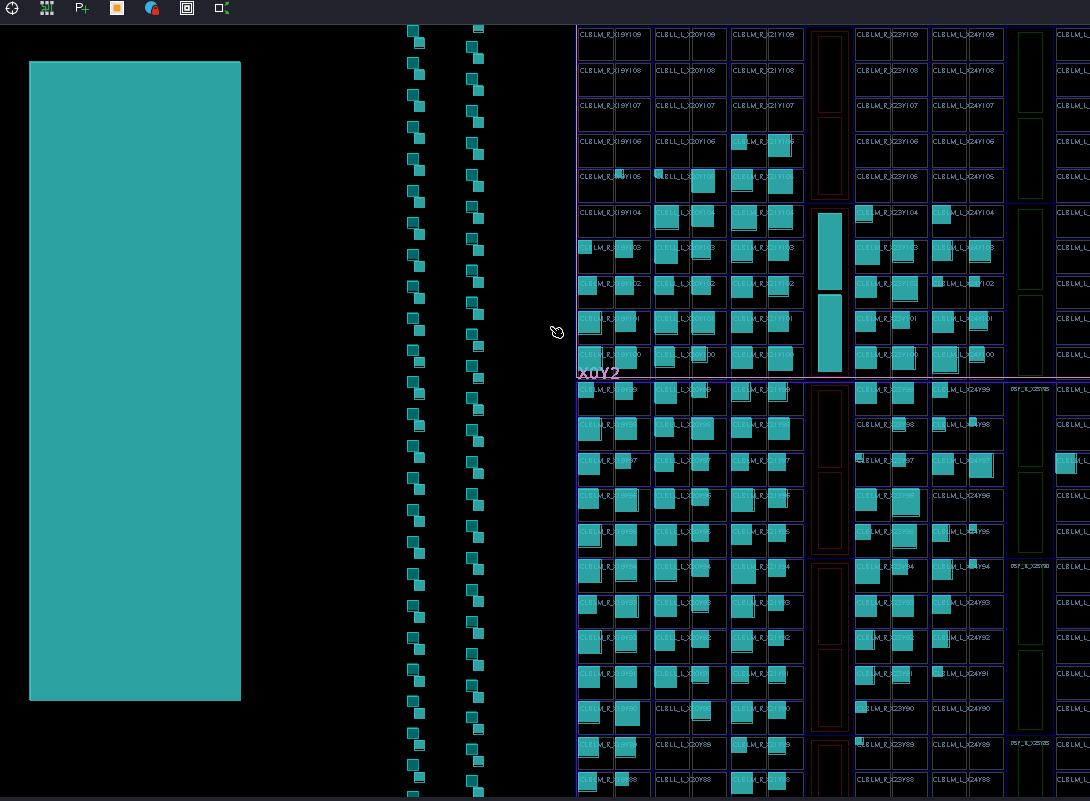
\includegraphics[width=0.95\textwidth]{fabric.png}
\caption{Fragment macierzy układu Zynq-7020 w~widoku „device” narzędzia Vivado:
komórki CLB (etykiety \texttt{CLBLM\_R}/\texttt{CLBLL\_L}) z~zajętymi zasobami
(turkus) oraz pionowe kolumny zasobów dedykowanych (BRAM/DSP).}
\label{fig:fabric}
\end{figure}

% =====================================================================
\section{Opis działania}

\textbf{Inicjalizacja.} Po starcie firmware wysyła rozkaz \texttt{ENABLE},
w~odpowiedzi na który logika nadaje trzy ramki konfiguracyjne MAX7219
(tabela~\ref{tab:max}): wyjście z~uśpienia, ustawienie skanowania 8~wierszy
oraz wyłączenie dekodowania. Następnie ustawiana jest domyślna jasność.

\textbf{Tryby pracy.} Aplikacja (\texttt{clock\_app.h}) działa jako automat
trzech stanów przełączanych przyciskiem środkowym (C):
\begin{itemize}[noitemsep]
    \item \texttt{MODE\_TIME} -- wyświetlanie bieżącego czasu; góra/dół
          zmienia jasność, lewy włącza/wyłącza alarm;
    \item \texttt{MODE\_SET\_TIME} -- nastawianie czasu; lewy/prawy wybiera
          pole godzin/minut, góra/dół modyfikuje wartość;
    \item \texttt{MODE\_SET\_ALARM} -- nastawianie czasu alarmu (analogicznie).
\end{itemize}
Wyjście z~trybu \texttt{SET\_TIME} zatwierdza nastawiony czas w~RTC.

\textbf{Miganie nastawianego pola.} Podczas nastawiania edytowane pole
(godziny lub minuty) miga z~okresem $250$~ms. Realizowane jest to programowo:
co \texttt{BLINK\_TICKS} iteracji pętli zmienia się faza migania i~w~fazie
wygaszonej odpowiednie znaki zastępowane są spacją przed wysłaniem na
wyświetlacz. Sprzętowo dostępny jest też rejestr „pozycji do migania”
(rozkaz \texttt{BLINK}), zgodny z~wymaganiem rejestru pozycji znaku.

\textbf{Alarm.} Raz na sekundę (\texttt{app\_second\_tick}) sprawdzane jest
dopasowanie bieżącego czasu do nastawionego alarmu. Aktywny alarm powoduje
miganie całego wyświetlacza oraz diody sygnalizacyjnej; dowolny przycisk
wycisza alarm.

\textbf{Potok renderowania.} Po zapisaniu nowej treści (\texttt{ASCII\_DATA})
i~rozkazie \texttt{ASCII}, automat PL przechodzi przez 8~wierszy: dla każdego
z~nich uruchamia \texttt{translator} (pobranie pikseli i~złożenie ramki),
oczekuje na gotowość, a~następnie zleca silnikowi szeregowemu wysłanie ramki
do matrycy. Mechanizm \texttt{abort} gwarantuje, że nowy rozkaz z~PS przerywa
trwającą transmisję, dzięki czemu obraz reaguje natychmiast na działania
użytkownika.

% =====================================================================
\section{Wnioski}

\begin{itemize}
    \item Zrealizowano kompletny system SoC zegara z~budzikiem, poprawnie
          dzieląc zadania między rdzeń ARM (logika aplikacji, RTC, klawiatura)
          a~logikę programowalną (dekodowanie ASCII i~transmisja szeregowa),
          co jest naturalnym i~efektywnym podziałem w~architekturze Zynq.
    \item Wstępne uruchomienie silnika MAX7219 na płycie Tang Nano~9K
          znacząco przyspieszyło prace -- protokół szeregowy zweryfikowano
          niezależnie od złożoności toru AXI, a~na Zynq przeniesiono już
          działający moduł.
    \item Stworzono testbenche w celu przetestowania działania poszczególnych modułów.
    \item Przerwanie sprzętowego timera (1~Hz) zapewniło dokładny i~niezależny
          od obciążenia pętli głównej pomiar czasu, a~maskowanie przerwania
          przy odczycie czasu wyeliminowało niespójności danych.
\end{itemize}

\end{document}
